\documentclass{beamer}

\usepackage{subfigure}
\usepackage{graphicx}
\usepackage{sidecap}
\usepackage{caption}
%\usepackage{subcaption}
\captionsetup{compatibility=false}
\usepackage{appendixnumberbeamer}
\usepackage{amsmath}
% --
\usepackage{multirow}
\usepackage{xcolor}
\usepackage{setspace}
\usepackage{hyperref}
\usepackage{anyfontsize}

\setbeamertemplate{footline}

\newenvironment{itemise} {\begin{itemize} \setlength{\itemsep}{0.2cm}} {\end{itemize}}
\usepackage[labelformat=empty]{caption}
\setbeamertemplate{sections/subsections in toc}[square]

%% COLORS
\definecolor{Gray}{gray}{0.9}
\definecolor{dblue}{rgb}{0.132,0.1,0.27}
\definecolor{mint}{cmyk}{1.0, 0.2, 0.6, 0.05}
\definecolor{ant}{cmyk}{0.5, 0.1, 0.0, 0.45}
\definecolor{lgray}{cmyk}{0.12, 0.0, 0.0, 0.17}
\definecolor{lred}{cmyk}{0.0, 0.9, 0.7, 0.0}


\usepackage{etoolbox}% http://ctan.org/pkg/etoolbox 
\usepackage{booktabs}

\newenvironment{literatur}{%
  \parskip2pt \parindent0pt \raggedright
  \def\lititem{\hangindent=0.5cm \hangafter1}}{%
  \par\ignorespaces}

\newcommand{\tb}[1]{{\color{blue}{\textbf{#1}}}}
\newcommand{\tm}[1]{{\color{mint}{\textbf{#1}}}}
\newcommand{\tr}[1]{{\color{red}{\textbf{#1}}}}

% Ilya: packages

\usepackage{tikz}
\usepackage{lmodern}
\usepackage{enumitem}

% Ilya: my commands

\newenvironment{mytemize}
{\vfill\itemize[nolistsep,itemsep=\fill,label=\color{blue}{$\triangleright$}]}
  {\enditemize}

\newcommand{\hitem}[1]{
  {\color{blue}{$\triangleright$}} 
  {#1} 
  {\hfill}
}

\setlist[itemize]{label= \color{blue}{$\triangleright$}}

\newcommand{\rarr}{$\Rightarrow$\ }


%\href{<Ziel>}{<Eingefasster Text>} 

%\logo{\includegraphics[height=0.7cm]{BdFlogo.eps}\hspace{300pt}\vspace{-5pt}}
%\logo{\includegraphics[height=0.8cm]{BdFlogo.eps}}
%\logo{\pgfputat{\pgfxy(-6.2,-0.5)}{\pgfbox[center,base]{\includegraphics[height=0.8cm]{BdFlogo.eps}}}}

%------------------------------------------------------------------------------------
% TITLE
%------------------------------------------------------------------------------------
\title[PSME]{Macroeconomics\\ Lecture 1 --- An Intro to Macro }
\author[I. Eryzhenskiy]{Ilya Eryzhenskiy}
\institute[BdF]{PSME Panth\'{e}on-Sorbonne Master in Economics}
\date[PSME macro]{Fall 2022}


%---BEGIN------------------------------------------------------------------------------
\begin{document}
%---BEGIN------------------------------------------------------------------------------
\begin{frame}
\maketitle
\end{frame}

%---FRAME------------------------------------------------------------------------------
\begin{frame}{%
\protect\hypertarget{macroeconomics-object-of-study}{%
Macroeconomics: objects}}

Main objects of study --- \emph{aggregate} measures of economic activity.
\vfill
Interactions of various \textbf{markets}\ldots{}
\vfill
\begin{columns}[c]
  \column{0.48\textwidth} 
  \begin{mytemize}
\item
  Goods:

  \begin{mytemize}
  \item
    Consumption goods
  \item
    Investment goods (capital)
  \end{mytemize}
\item
  Services
  \end{mytemize}
  \column{0.48\textwidth} 
\begin{mytemize}
 
\item
  Labor
\item
  Finance:

  \begin{mytemize}
   
  \item
    Banking
  \item
    Market finance
  \end{mytemize}
\item
  Currency
\end{mytemize}

\end{columns}
\vfill
\ldots{}and \textbf{policies}: 
\vfill
\ 
\hitem{Monetary}
\hitem{Fiscal}
\hitem{Regulation}
\\
\vfill
One (even huge) market is not ''macro`` enough: e.g. real estate

\end{frame}

\begin{frame}{Macroeconomics: motivation}

  Why care for the macro-economy?
  \vfill
\begin{mytemize}
\item As \tb{households}, we are all affected: 
  \begin{mytemize}
  \item Crises \rarr unemployment: lives depend on business cycles
  \item Need to check macro for big decisions: housing, retirement, own business\ldots
  \end{mytemize}
\item \tb{Businesses}: cycles influence demand and supply chains, interest rates, exchange rates, inflation\ldots
\item \tb{Policymakers}: macro policy has proven to be influential. In addition, people tend to (over-)associate macro phenomena with politics \rarr pressure on politicians
\end{mytemize}
\end{frame}

\begin{frame}{%
\protect\hypertarget{macroeconomics-rules-keynes}{%
Macroeconomics rules: Keynes}}

\begin{quote}
Practical men who believe themselves to be quite exempt from any
intellectual influence, are usually the slaves of some defunct
economist.
\end{quote}

\begin{flushright}
John Maynard Keynes
\end{flushright}

\vfill
\textit{N. B.}: Keynes \textit{is} the most influential macroeconomist to date\ldots
\end{frame}
%---FRAME------------------------------------------------------------------------------
\begin{frame}{What are business cycles?}

  Historically, Smith, Marx, Kondratiev and others thought of cycles literally --- economic indicators following sine waves
  \vfill
  Famous example (not macro) --- pork cycles:
  \vfill
\begin{center}
\begin{figure}[h!]
	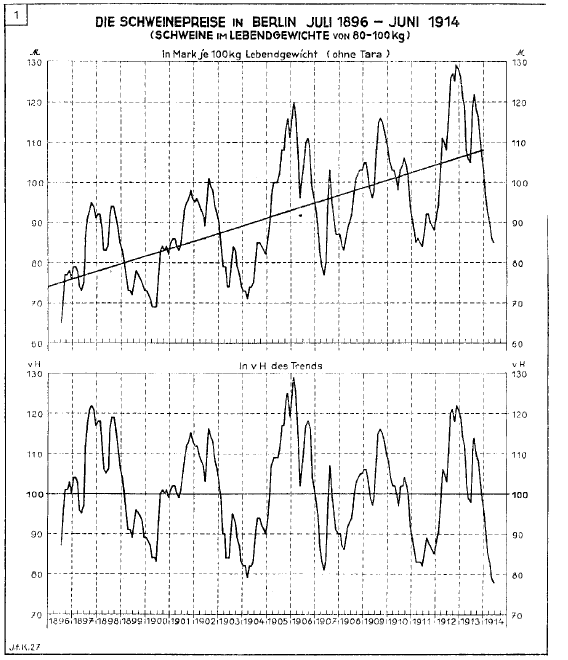
\includegraphics[clip,width=0.4\textwidth]{FIGURES/1_PorkCycle_a}
\caption{Pork prices in Berlin, July 1896 - June 1914}
%	\label{fig:GPD} 
\end{figure}
%\vspace{-2mm}
%\begin{minipage}{1.0\columnwidth}
%\tiny	
%%\textbf{Note.} .\\
% \textbf{Source.} von Hanau, Arthur (1928) 'Die Prognose der Schweinpreise', in: \emph{Vierteljahreshefte zur Konjunkturforschung}, Sonderheft 7. Berlin: Institut f\"{u}r Konjunkturforschung, \href{https://www.diw.de/documents/dokumentenarchiv/17/diw_01.c.43353.de/viertel_1928.pdf}{[Link]}.\\
%\end{minipage}
\end{center}

\end{frame}
%---FRAME------------------------------------------------------------------------------
%---FRAME------------------------------------------------------------------------------
%\begin{frame}{Income and Output}
%
%\begin{mytemize}
%{\footnotesize
%\item \tb{Gross domestic product} (GDP): \emph{Indicator of the goods and services produced within an economy in a year for final use, a nation's economic well-being.}
%}
%\end{mytemize}
%\vspace{-5mm}
%\begin{center}
%\begin{figure}[h!]
%	\subfigure{\includegraphics[clip,width=0.95\textwidth]{../PSME_stata/FIGURES/1_GDP}
%	}      
%%	\label{fig:GPD} 
%\end{figure}
%\vspace{-2mm}
%\begin{minipage}{0.9\columnwidth}
%\tiny	
%%\textbf{Note.} .\\
% \textbf{Source.} Jorda-Schularick-Taylor Macrohistory Database \href{http://www.macrohistory.net/data/}{[Link]} .\\
%\end{minipage}
%\end{center}
%
%\end{frame}
%---FRAME------------------------------------------------------------------------------
%\begin{frame}{Trend vs. cycle}
%
%\begin{mytemize}
%\item Steady trend in \tb{economic growth} (GDP) over time.
%\item Recurring fluctuations of GDP around its trend ($\rightarrow$\tb{business cycle})
%\end{mytemize}
%
%\begin{center}
%\begin{figure}[h!]
%	\subfigure{\includegraphics[clip,width=0.95\textwidth]{../PSME_stata/FIGURES/1_GDPtrendcycle}
%	}      
%%	\label{fig:GPD} 
%\end{figure}
%\vspace{-2mm}
%\begin{minipage}{0.9\columnwidth}
%\tiny	
%\textbf{Note.} Trend-cycle decomposition using a Hodrick-Prescott filter with a smoothing value of 6.25.\\
% \textbf{Source.} Own calculations. Jorda-Schularick-Taylor Macrohistory Database.\\
%\end{minipage}
%\end{center}
%
%\end{frame}
%---FRAME------------------------------------------------------------------------------
\begin{frame}{Towards modern business cycles}

\begin{mytemize}
\item \tb{National Bureau of Economic Research} (NBER), founded 1920, influential group of economists
\item Persuaded that statistical methods make study of economic phenomena (cycles) possible
\item Idea by Arthur Burns \& Wesley Mitchell:
\begin{mytemize}
\item Focus on boom and bust periods $\Leftrightarrow$ peaks and troughs of cycle
\item Identify common patterns for different booms and busts
\end{mytemize}
%\item NBER still influential in macroeconomics. See working papers: \tiny
%  \begin{mytemize}
%  \item \url{https://www.nber.org/programs-projects/programs-working-groups/economic-fluctuations-and-growth?page=1&perPage=50}
%  \end{mytemize}
\end{mytemize}

\end{frame}

\begin{frame}{Burns-Mitchell Diagrams: an example}

\begin{columns}
          \column{0.50\linewidth}
             \centering
             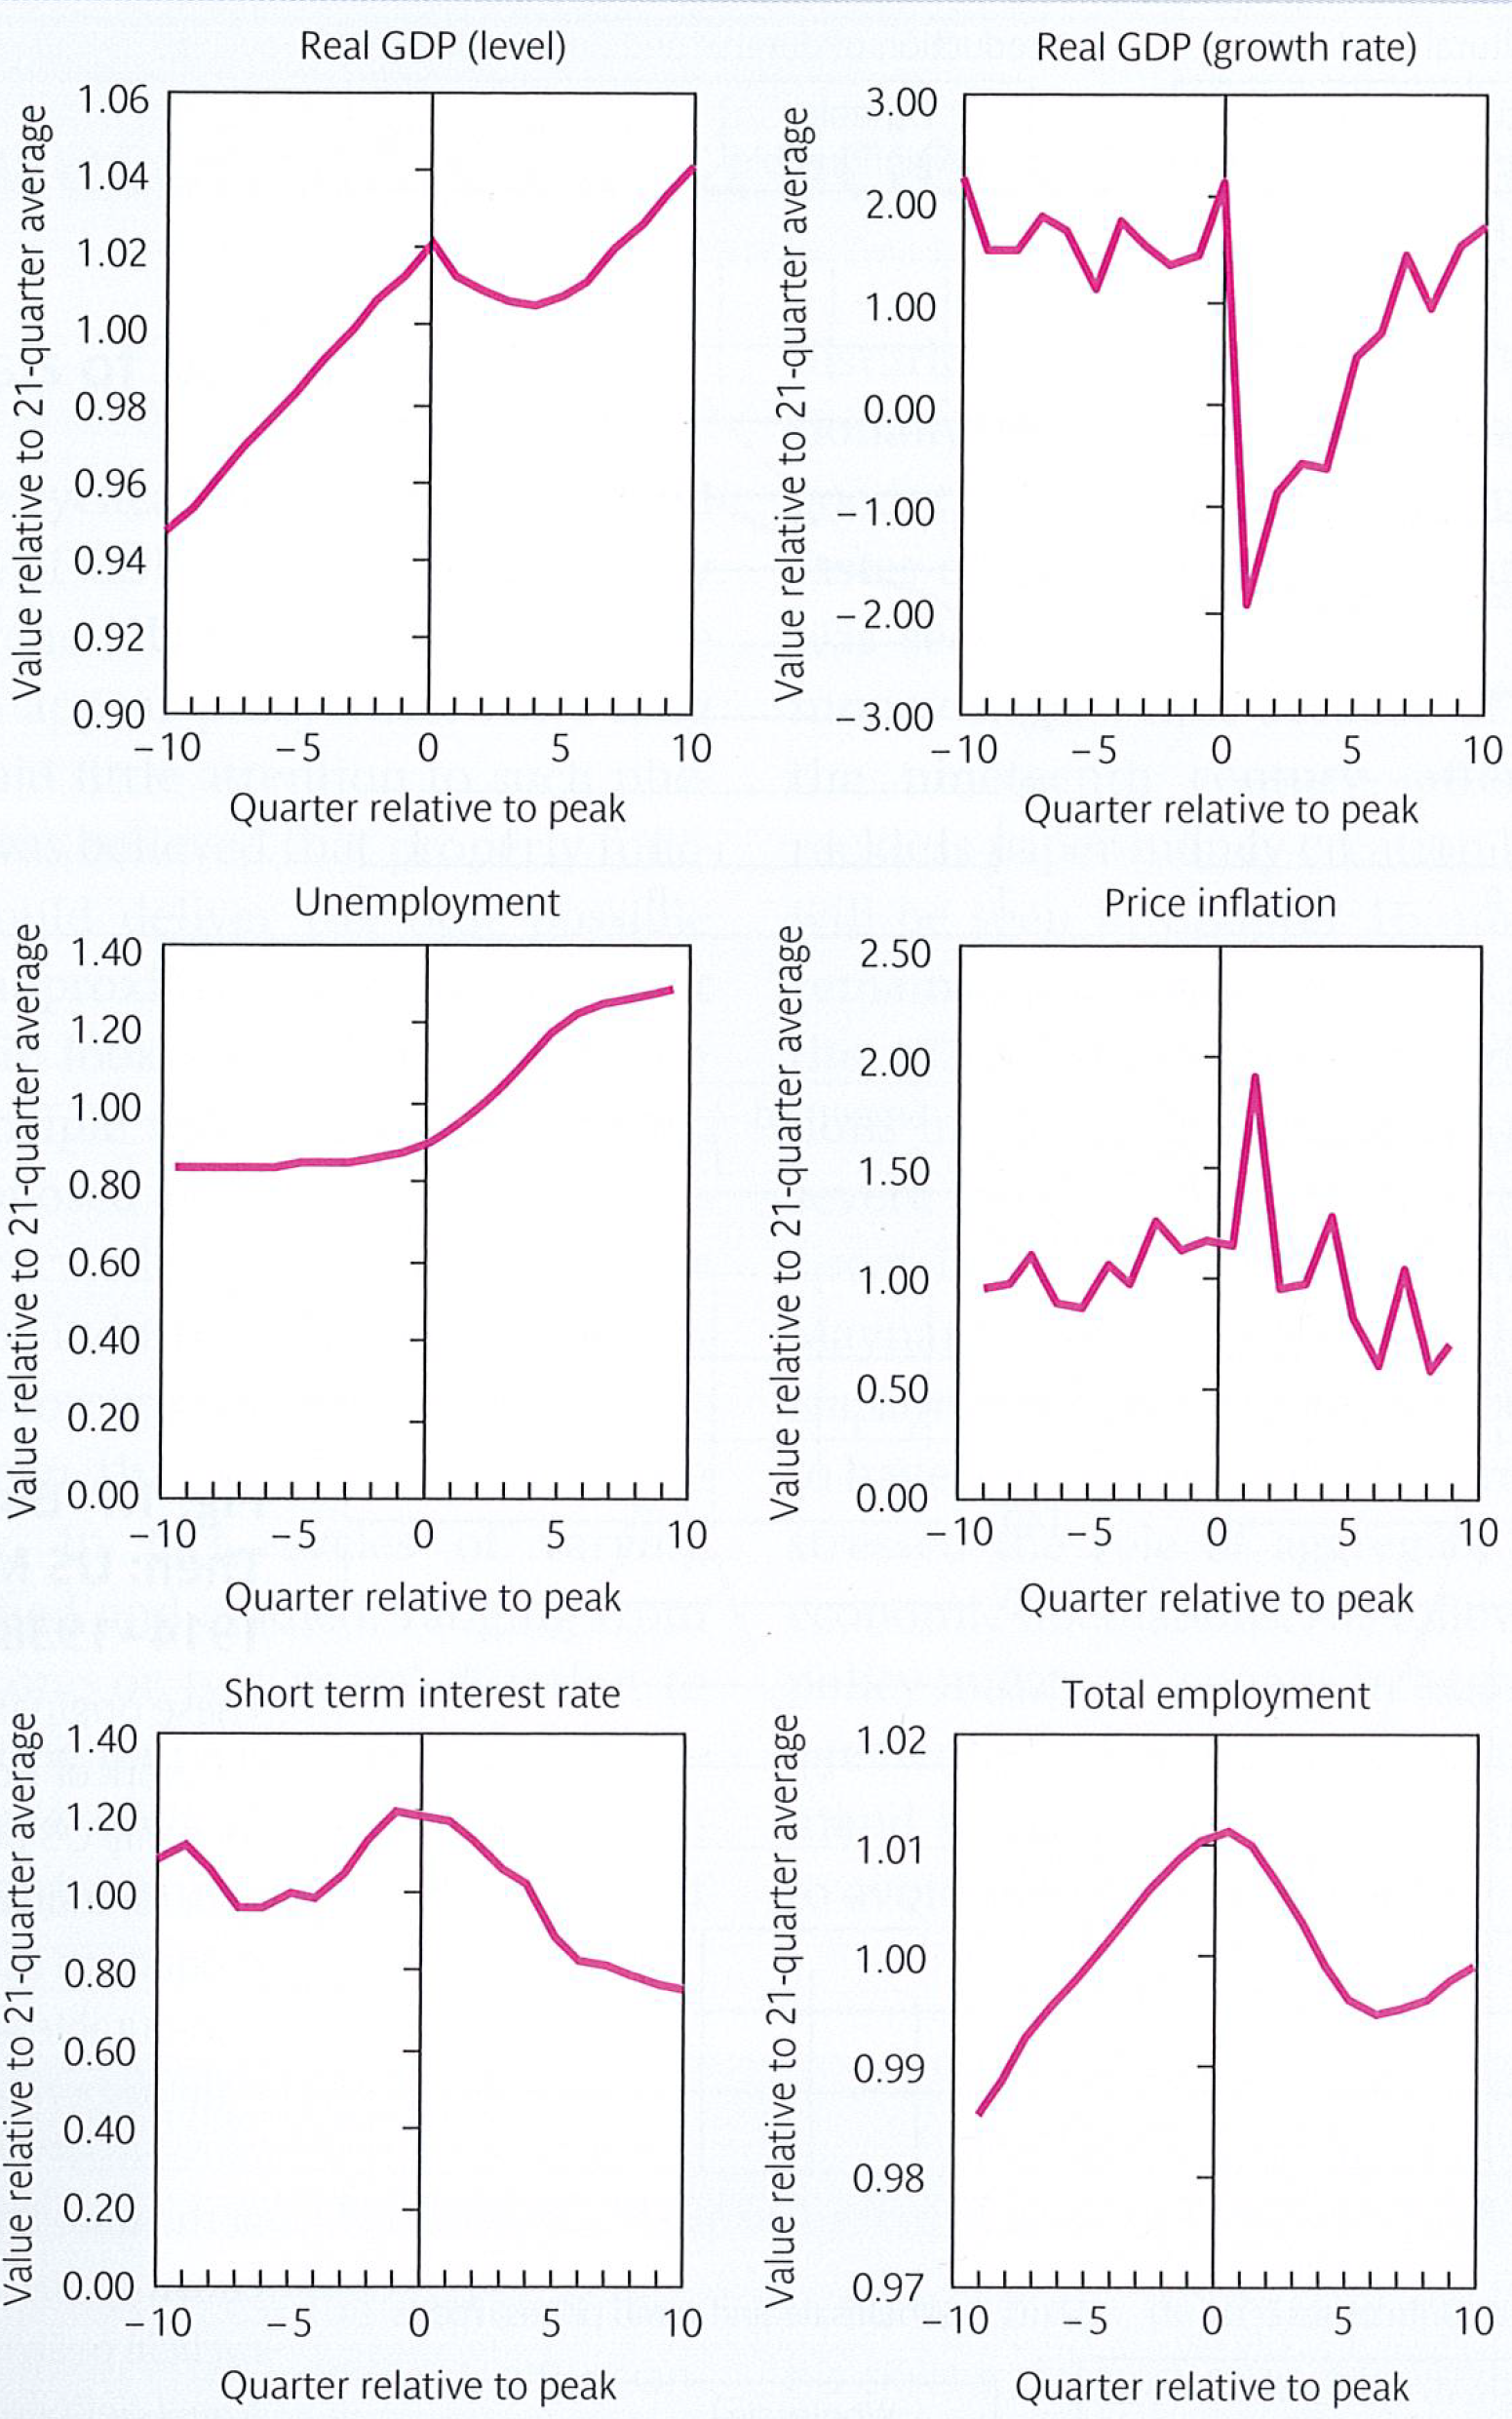
\includegraphics[clip,width=0.8\columnwidth]{FIGURES/1_BurnsMitchell_b}
           \vspace{-2mm}
	\begin{minipage}{1.0\columnwidth}
%	\tiny	
%	\textbf{Note.} The Figure shows the average behaviour of variables around cyclical peaks in eight countries.\\
% 	\textbf{Source.} Burda and Wyplosz (2013), Figure 1.6 (p. 13).\\
	\end{minipage}
	% COLUMN(2)
    \column{0.50\linewidth}
           
\begin{mytemize}
\item peak of GDP = vertical line
\item Unemployment = \tb{countercyclical}
\item Inflation = procyclical (\textbf{\emph{lagging}} the cycle)
\item Short term interest rate, employment = \tb{procyclical}
\end{mytemize}


%	\begin{minipage}{0.9\columnwidth}		
%	\tiny
%	\begin{singlespace*}
%	$^*$ The peak is determined using a procedure proposed by Harding and Pagan (2001) 'Dissecting the Cycle: A Methodological investigation', \emph{Journal of Monetary Economics}, 49(2); see Burda \& Wyplosz Box 1.1 for methodological details.          	
%	\end{singlespace*}
%	\end{minipage}
	
	
\end{columns} 
	       

\end{frame}

\begin{frame}{Recession dating by NBER}
  \centering
             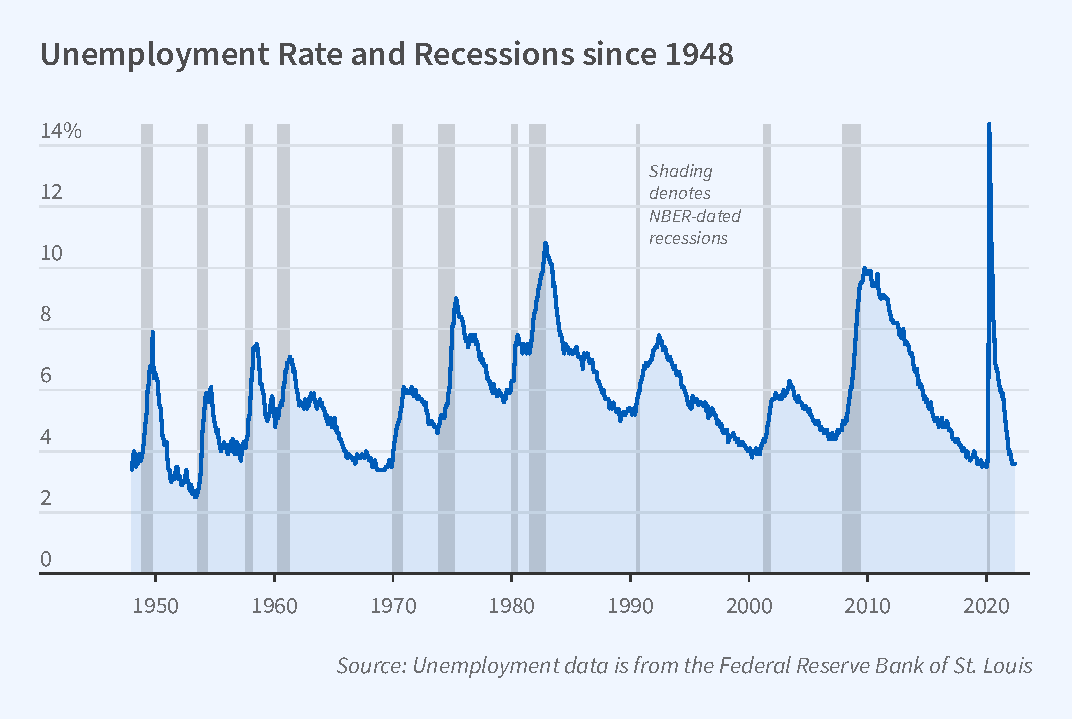
\includegraphics[width=0.9\textwidth]{FIGURES/nber_unemp_aft1948}
\end{frame}
%---FRAME------------------------------------------------------------------------------
%---FRAME------------------------------------------------------------------------------
\begin{frame}{Methodology of Macroeconomics: Theory}

\begin{mytemize}
\item Macro deals with complex relationships of dynamic variables
\item Theory with a good deal of \textit{abstraction} necessary:
\begin{mytemize}
\item \tb{exogenous} variables are taken as given, ``out of nowhere''
\item \tb{endogenous} variables are explained by the model
\end{mytemize}
\end{mytemize}

\begin{center}
\begin{figure}[h!]
	\subfigure{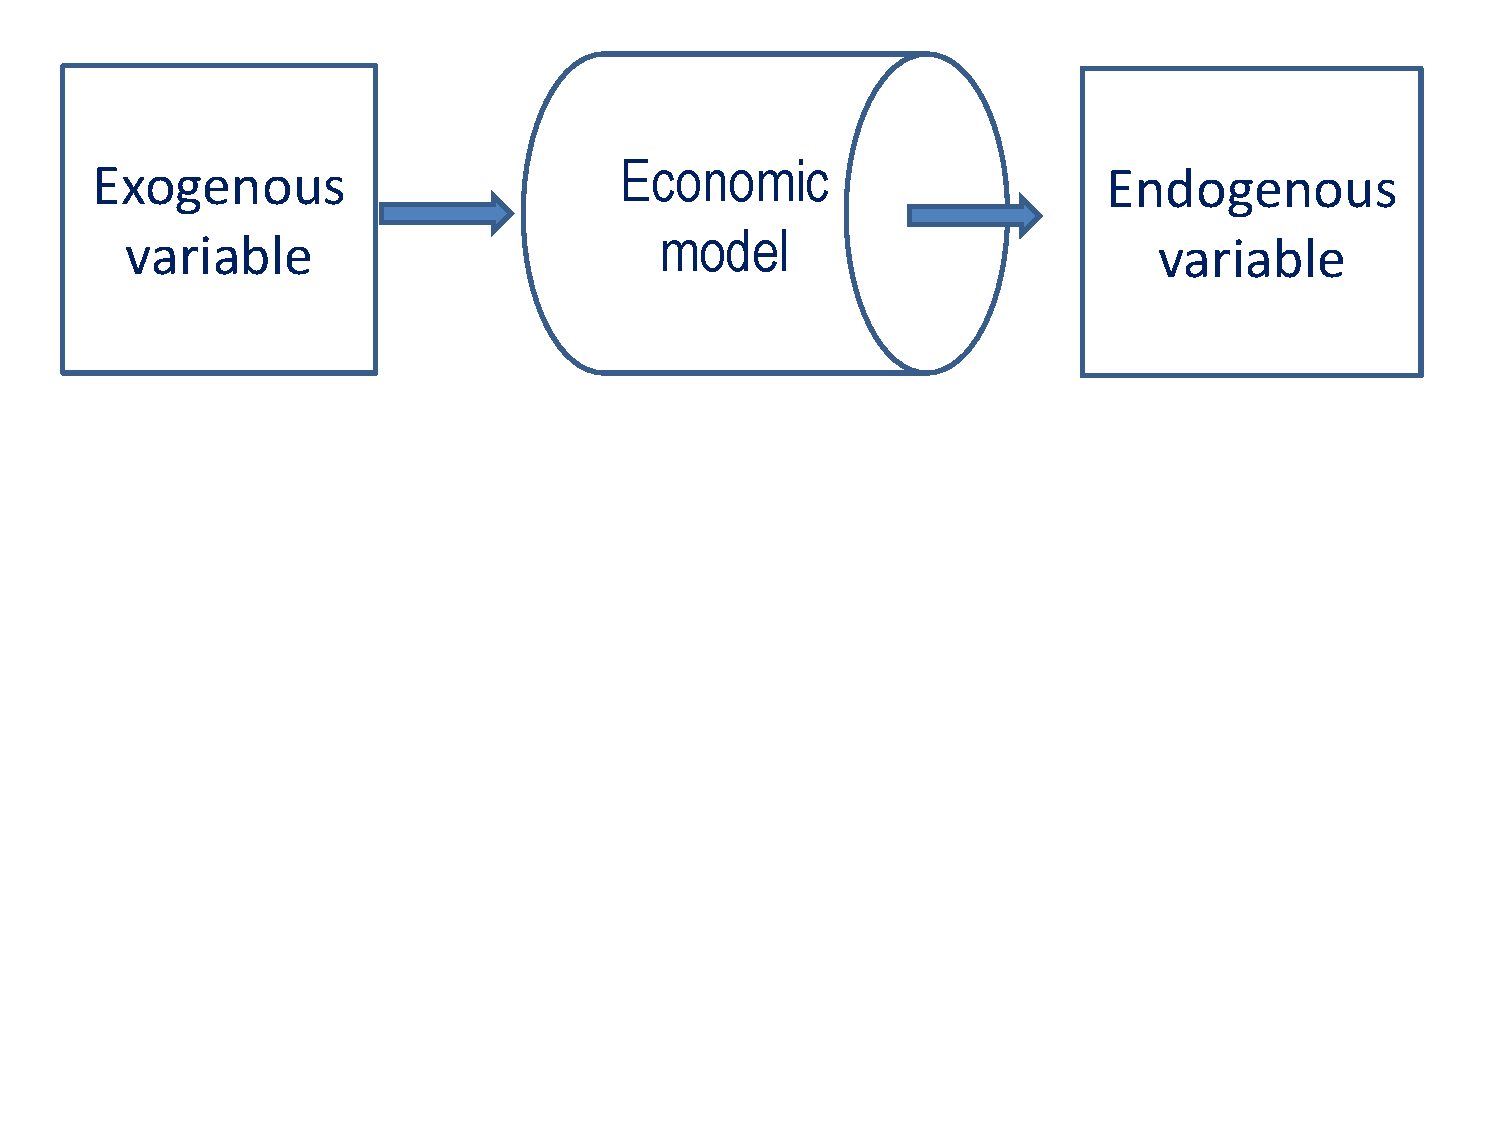
\includegraphics[trim=0 300 0 0,clip,width=0.7\textwidth]{FIGURES/1_EconModel}
	}      
	%[trim=left bottom right top
%	\label{fig:GPD} 
\end{figure}
%\vspace{-2mm}
%\begin{minipage}{0.9\columnwidth}
%\tiny	
%\textbf{Note.} .\\
% \textbf{Source.} Jorda-Schularick-Taylor Macrohistory Database \href{http://www.macrohistory.net/data/}{[Link]} .\\
%\end{minipage}
\end{center}

\end{frame}
% baby background:
{
\usebackgroundtemplate%
{%
  %\begin{figure}[b!]
  \begin{tikzpicture}
	\draw node[opacity=0] at (15,6) {
\includegraphics[width=0.3\paperwidth]{baby_logo.png}};%
    \draw node[opacity=0.3] at (14.5,-0.4) {
\includegraphics[width=0.3\paperwidth]{baby_logo.png}};%
    %\draw node[opacity=0.8] at (15.3,6) {\includegraphics[width=0.23\paperwidth]{../PSE_logo.png}};%
	\draw node[opacity=0] at (10.3,-1.4) {
\includegraphics[width=0.37\paperwidth]{baby_logo.png}};%
	\draw node[opacity=0] at (6,-1.4) {
\includegraphics[width=0.3\paperwidth]{baby_logo.png}};%
  \end{tikzpicture}
  %\end{figure}
}
\begin{frame}{Models can be fun}
   Macroeconomic crises and monetary policy can be seen on a real-life historical example of\ldots a \tb{baby-sitters cooperative} 
\vfill
  \begin{itemize}
	\item Parents babysit each others' children
	  \vfill
	\item A currency --- \textit{scrpis} --- introduced to promote fairness
	  \vfill
	  \begin{itemize}
		\item 1 \textit{scrip} $=$ 1 hour of baby-sitting
	  \vfill
	\item rigid price set \textit{exogenously}, rather than \textit{endogenously} determined by market
	  \vfill
	\item each family receives a number of scrips to begin with
	  \vfill
	  \end{itemize}
	  \vfill
		\item if a couple wants more babysitting for their child, need to babysit more
	  \vfill
	\item some have busy periods: cannot babysit, but need babysitting $\Rightarrow$ need excess \textit{reserves} of scrips
  \end{itemize}
  Source: Joan and Richard Sweeney ``Monetary Theory and the Great Capitol Hill Baby-Sitting Co-op Crisis.'' Journal of Monetary Economics, 1978.
\end{frame}
\begin{frame}{A crisis}
  \begin{itemize}
	\item Some babysitting-scripts accounting problems $\Rightarrow$ an episode with a decrease of scrips in circulation: an \tr{exogenous shock} 
	  \vfill
	\item parents worried they don't have enough reserve scrips and reduce spending\ldots 
	  \vfill
	\item \ldots others have less scrips, worried they don't have enough, and so on
	  \vfill
	  \begin{itemize}
		\item A vicious cycle / \textit{coordination failure} / bad \textit{equilibrium}
	  \end{itemize}
	  \vfill
	\item a monetary problem (exogenous) causing a decline of activity (endogenous): babysitting has stopped
  \end{itemize}
\end{frame}
}
%---FRAME------------------------------------------------------------------------------
\begin{frame}{Methodology of Macroeconomics: Data}


\begin{mytemize}
\item Unrealistic models are fine as long they:
  \begin{mytemize}
	\item Give novel insights (M. Friedman)
	\item Are \textit{falsifiable} --- can be proven wrong (K. Popper)
  \end{mytemize}
\item Confronting macro \tb{theories} with \tr{data} is challenging:
\begin{mytemize}
\item aggregate indices: measurement problems
\item how to separate correlation and causality? Natural experiments, as in applied micro, are hard to find
\item expectations are crucial, but never directly measurable
\end{mytemize}
\item Solutions:
\begin{mytemize}
\item complex reduced form econometrics --- VAR (Nobel prize of C. Sims) 
\item output of calibrated or estimated models (involving expectations) to be compared to reduced-form estimates: importance of \tb{impulse response} analysis
\end{mytemize}
\end{mytemize}

\end{frame}

{
\usebackgroundtemplate%
{%
  %\begin{figure}[b!]
  \begin{tikzpicture}
	\draw node[opacity=0] at (15,6) {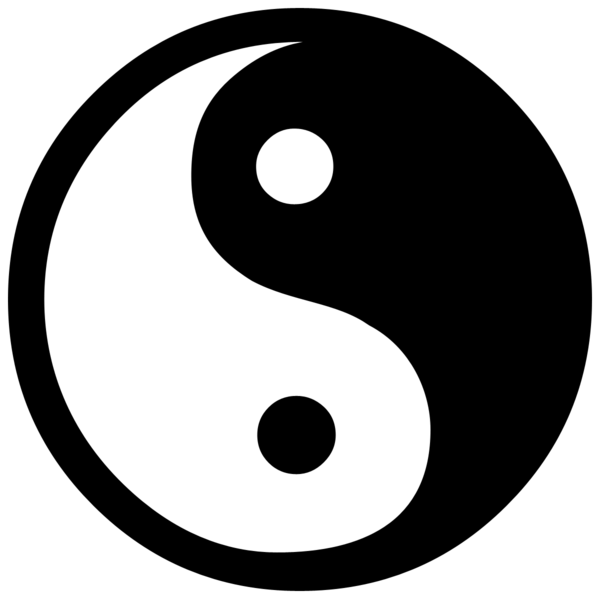
\includegraphics[width=0.3\paperwidth]{FIGURES/yin_yang.png}};%
    \draw node[opacity=0.15] at (14.5,-0.4) {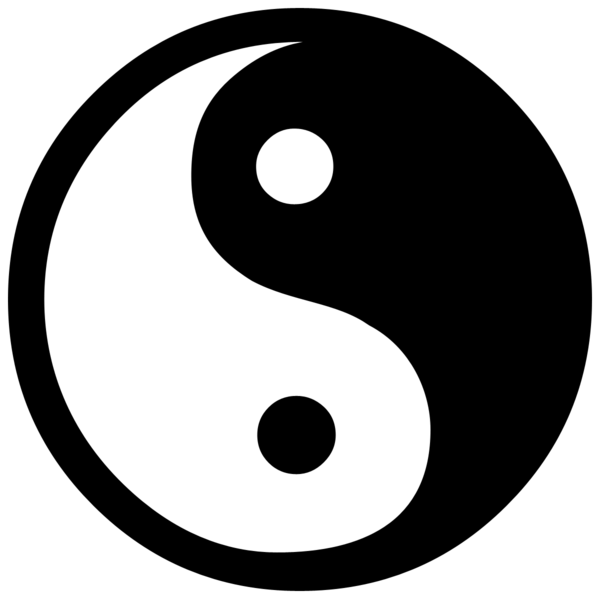
\includegraphics[width=0.3\paperwidth]{FIGURES/yin_yang.png}};%
    %\draw node[opacity=0.8] at (15.3,6) {\includegraphics[width=0.23\paperwidth]{../PSE_logo.png}};%
	\draw node[opacity=0] at (10.3,-1.4) {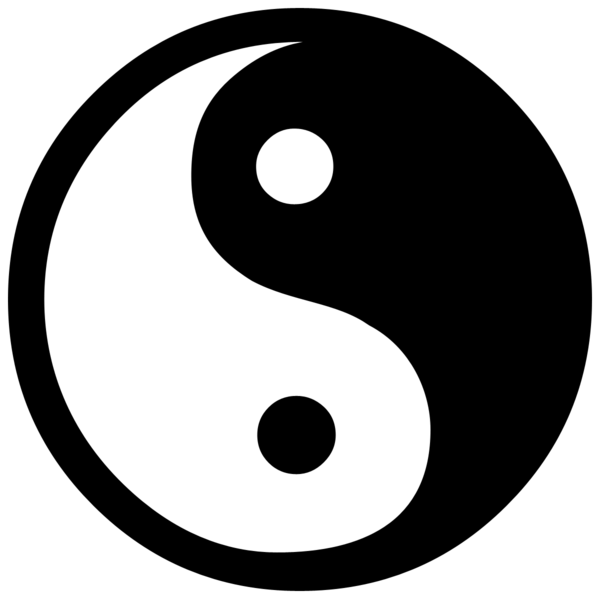
\includegraphics[width=0.37\paperwidth]{FIGURES/yin_yang.png}};%
	\draw node[opacity=0] at (6,-1.4) {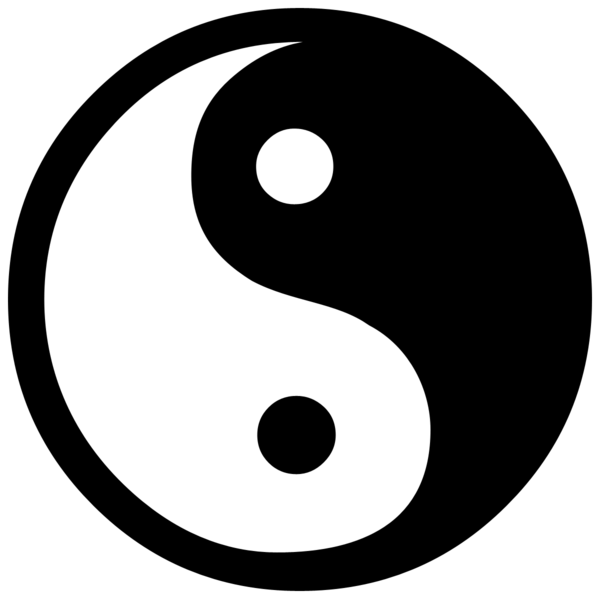
\includegraphics[width=0.3\paperwidth]{FIGURES/yin_yang.png}};%
  \end{tikzpicture}
  %\end{figure}
}
\begin{frame}{Macro dichotomies}
  		\begin{center}
		  \underline{\textbf{Macroeconomics}}\\
				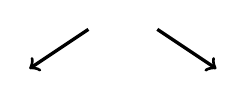
\begin{tikzpicture}[xscale = .5, yscale = .5]
				  \draw[->, very thick] (-0.5, 1)--(-2, 0) ;
		\draw[->, very thick] (1.25, 1)--(2.75, 0) ;
		\end{tikzpicture}
		\end{center}
		\begin{columns}[T]
				\column{.48\textwidth}
				\centering
			  \underline{\textbf{Theoretical}}
				\begin{itemize}
				  \item A zoo of models (see next slides)
				  \item \tb{Focus for this course}
				\end{itemize}
\column{.48\textwidth} 
				\centering
\underline{\textbf{Empirical}}
				\begin{itemize}
					\item Model estimation
					  \begin{itemize}
						  \item 
							introduction with practical implementation (coding) \tr{in TD}
						\end{itemize}
				  \item VAR 
					\begin{itemize}
						\item see Econometrics class
					  \end{itemize}
				\end{itemize}
				\end{columns}
		\vfill
\end{frame}


\begin{frame}{Macro dichotomies}
  		\begin{center}
		  \underline{\textbf{Macroeconomic models}}\\
				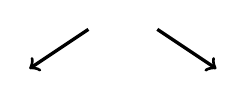
\begin{tikzpicture}[xscale = .5, yscale = .5]
				  \draw[->, very thick] (-0.5, 1)--(-2, 0) ;
		\draw[->, very thick] (1.25, 1)--(2.75, 0) ;
		\end{tikzpicture}
		\end{center}
		\begin{columns}[T]
				\column{.48\textwidth}
				\centering
			  \underline{\textbf{Short-run}}
				\begin{itemize}
				  \item Most of macroeconomists' job. Why?
					\begin{itemize}
					  \item Immediately applicable?
					  \item Most politicians' focus?
					\end{itemize}
				  \item \tb{Focus of this course}
				\end{itemize}
\column{.48\textwidth} 
				\centering
\underline{\textbf{Long-run}}
				\begin{itemize}
				  \item More substantial problems
				  \item See Growth course (unless you are in financial track!)
				\end{itemize}
				\end{columns}
		\vfill
\end{frame}
\begin{frame}{Macro dichotomies}
  		\begin{center}
		  \underline{\textbf{Macroeconomic models}}\\
				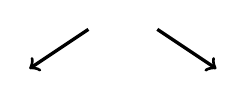
\begin{tikzpicture}[xscale = .5, yscale = .5]
				  \draw[->, very thick] (-0.5, 1)--(-2, 0) ;
		\draw[->, very thick] (1.25, 1)--(2.75, 0) ;
		\end{tikzpicture}
		\end{center}
		\begin{columns}[T]
				\column{.48\textwidth}
				\centering
			  \underline{\textbf{Dynamic}}
				\begin{itemize}
				  \item The modern approach
				  \item \tb{Most of the course}
				\end{itemize}
\column{.48\textwidth} 
				\centering
\underline{\textbf{Static}}
				\begin{itemize}
				  \item Keynes-Hicks heritage (20th century)
				  \item \tr{Beginning of course} 
				\end{itemize}
				\end{columns}
		\vfill
\end{frame}

\begin{frame}{Macro dichotomies}
  		\begin{center}
		  \underline{\textbf{Macroeconomic models}}\\
				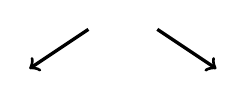
\begin{tikzpicture}[xscale = .5, yscale = .5]
				  \draw[->, very thick] (-0.5, 1)--(-2, 0) ;
		\draw[->, very thick] (1.25, 1)--(2.75, 0) ;
		\end{tikzpicture}
		\end{center}
		\begin{columns}[T]
				\column{.48\textwidth}
				\centering
			  \underline{\textbf{Closed economy}}
				\begin{itemize}
				  \item Wild simplification, but\dots
				  \item \dots most macro scholars based in the U.S. --- large and independent enough \rarr closed economy is 
					most studied model
				  \item \tb{Most of the course}
				\end{itemize}
\column{.48\textwidth} 
				\centering
\underline{\textbf{Open economy}}
				\begin{itemize}
				  \item Small open economy models: country as \textit{price-taker}
				  \item Large open economy models: country influences prices
				  \item Will see both \tr{occasionally} in the course
				\end{itemize}
				\end{columns}
		\vfill
\end{frame}

\begin{frame}{Macro dichotomies}
  		\begin{center}
		  \underline{\textbf{Macroeconomic models}}\\
				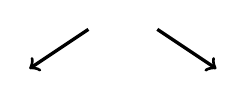
\begin{tikzpicture}[xscale = .5, yscale = .5]
				  \draw[->, very thick] (-0.5, 1)--(-2, 0) ;
		\draw[->, very thick] (1.25, 1)--(2.75, 0) ;
		\end{tikzpicture}
		\end{center}
		\begin{columns}[T]
				\column{.48\textwidth}
				\centering
				\underline{\textbf{Flexible price (neoclassical)}}
				\begin{itemize}
				  \item Usually result in optimal allocations
					\begin{itemize}
					  \item \textit{laissez-faire} economics
					  \end{itemize}
					  \item Useful to understand how a perfect world would work --- normative approach
				  \item \tb{Most of the course}
				\end{itemize}
\column{.48\textwidth} 
				\centering
				\underline{\textbf{Sticky price (Keynesian)}}
				\begin{itemize}
				  \item Associated with corrective interventions, such as Keynesian demand management
				  \item \tr{Beginning} and \tr{middle} of course
				\end{itemize}
				\end{columns}
		\vfill
\end{frame}

 
}
\end{document}

